% 压强体积图
% 理想气体|做功|压强|体积|状态方程

\begin{issues}
\issueDraft
\end{issues}

\pentry{功\upref{Fwork}}

\begin{figure}[ht]
\centering
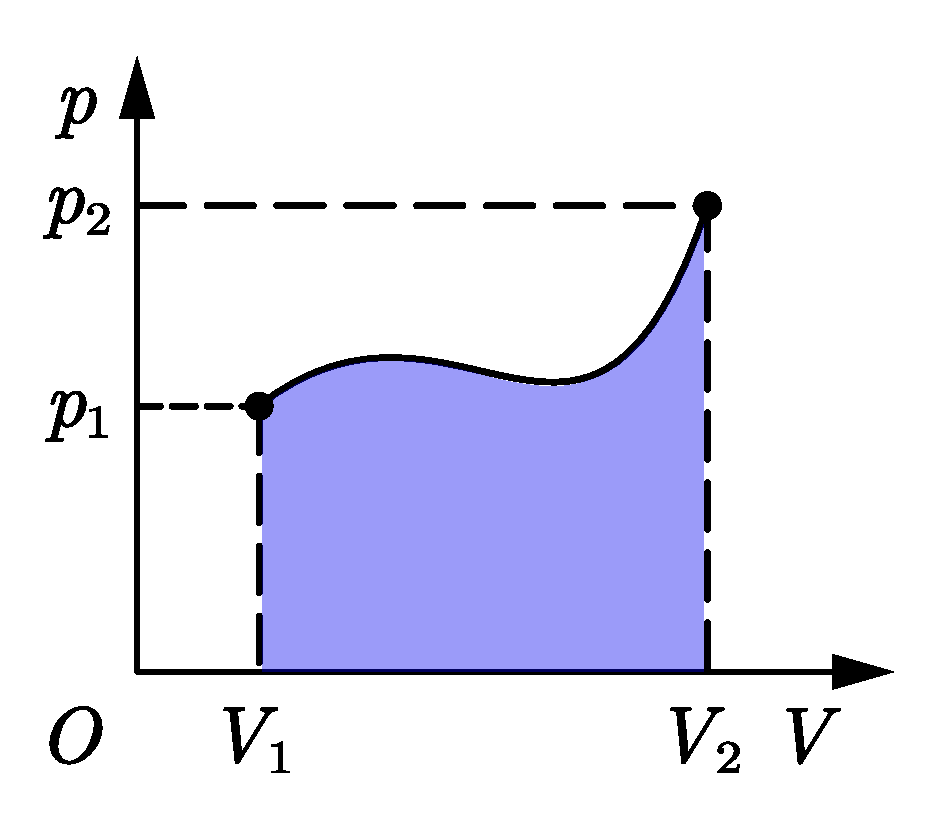
\includegraphics[width=5cm]{./figures/PVgraf_1.pdf}
\caption{$p-V$图中气体做的功} \label{PVgraf_fig1}
\end{figure}

如\autoref{PVgraf_fig1} 所示,做功
\begin{equation}\label{PVgraf_eq1}
W = \int_{V_1}^{V_2}P(V) \dd{V}
\end{equation}

做功就是 $p-V$ 曲线下面的面积. 

\begin{figure}[ht]  
\centering
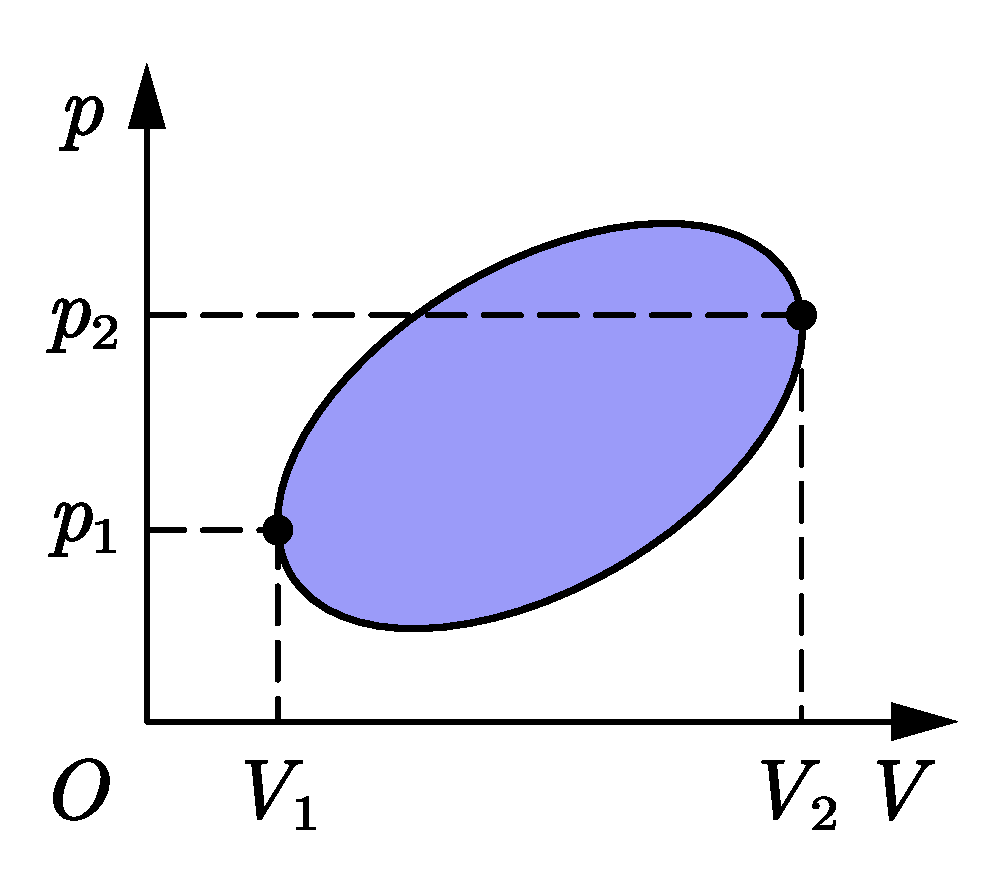
\includegraphics[width=5cm]{./figures/PVgraf_2.pdf}
\caption{$p-V$图中闭合路径气体做的功} \label{PVgraf_fig2}
\end{figure}

如\autoref{PVgraf_fig2} 所示,如果是一个闭合路径, 那么对外做功就是闭合路径围出的面积(顺时针为正).

如果是容器中的理想气体, 可以画出等温曲线. 这样理想气体状态方程中的三个量都可以从图中看出.
  